\section{Motivation}

Robotics is understood as an important area of research within Engineering and Computer Science, optimizing and automating various areas of industry. One of the ways in which research is developed in this area is in robot soccer, since it comprises challenges of machine perception, environment modeling, planning and reasoning, control, and multiagent strategy.

Over the years, several techniques have been developed to address each of the problems related to robot soccer, based on the theory of Signal Processing, Control, Trajectory Planning, and classical Artificial Intelligence. These techniques have proved to be functional for maturing the challenge. However, such techniques still perform worse as compared to humans in these activities.

In recent years, however, with the development of processing and memory architectures, Machine Learning techniques have been able to achieve or even have surpassed the human performance in machine perception activities (Computer Vision \cite{DBLP:journals/corr/LuT14} and Speech Recognition \cite{DBLP:journals/corr/XiongDHSSSYZ16a}), by planning and reasoning \cite{DBLP:journals/corr/abs-1712-01815}, as shown in Figure \ref{alphazero}, and also by controlling agent locomotion \cite{DBLP:journals/corr/HeessTSLMWTEWER17}, as shown in Figure \ref{locomotion}. In this way, the learning field of combining techniques from Deep Learning and Reinforcement Learning appears as a great candidate in the search of General Artificial Intelligence.


\begin{figure}[ht]
\centering
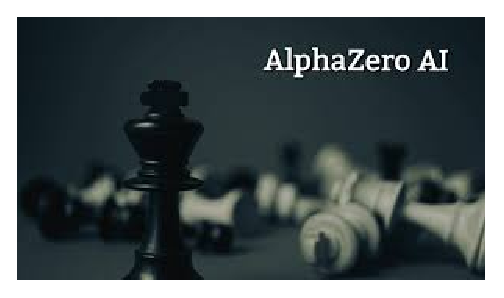
\includegraphics[width=0.6\textwidth]{Cap1/AlphaZero}
\caption{AlphaGo Zero, learning model that beat the best players of Go, Chess and Shogi, learning to play without previous human knowledge \cite{DBLP:journals/corr/abs-1712-01815}.}
\label{alphazero}
\end{figure}



\begin{figure}[ht!]
\centering
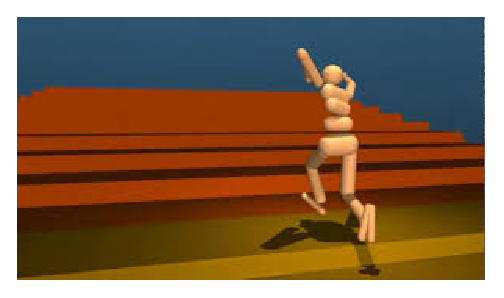
\includegraphics[width=0.6\textwidth]{Cap1/Locomotion}
\caption{Locomotion of Agent via Deep Reinforcement Learning \cite{DBLP:journals/corr/HeessTSLMWTEWER17}.}
\label{locomotion}
\end{figure}


\section{Contextualization}

RoboCup is an international scientific community aiming to advance the state of the art of intelligent robots. Its mission is that a team of robots will be able to beat the human team champion of the World Cup until the year 2050 \cite{10.1007/3-540-64473-3_46}. Since this is a goal with a range of different challenges to be solved, there are several categories of competition within the community.

In Robocup Soccer 3D Simulation League, as shown in Figure \ref{soccer3d}, there is a robot soccer competition in which each team has eleven Nao robots in a physical simulation environment called Simspark \cite{simspark2005}. The purpose in this case is to create and improve algorithms and physical models for the perception, locomotion, and strategy of the humanoid robot, before actually shipping them into hardware for real-world evaluation.

\begin{figure}[ht!]
\centering
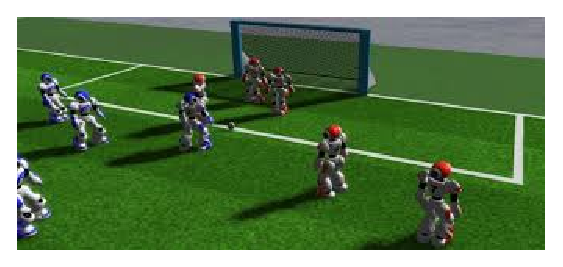
\includegraphics[width=0.6\textwidth]{Cap1/Soccer3D}
\caption{A Snapshot from the RoboCup Soccer 3D Simulation League.}
\label{soccer3d}
\end{figure}

Over the last few years, team efforts have been seen in three different areas, layers, or strands. The first area is considered more basic, meaning the construction of the agent that can model the environment and interact with it -- involving both the construction of a solid software architecture and the application of traditional techniques of localization and control of the humanoid robot \cite{AI1110-macalpine}.

The second layer, explored at the highest level, involves creating behaviors to perform actions within the game, given the modeled environment -- from the creation of models and heuristics for navigation to the creation of multiagent strategies for positioning and marking \cite{LNAI16-MacAlpine}.

The third strand, to be approached in this work, is the creation and optimization of models based upon learning for activities such as robot walking and kicking. Simulated categories have great value for learning test, mainly because they provide a benchmark for comparison and do not involve physical robots. Historically, teams with the best performance in these two issues are usually the best positioned within category competitions, due to the fact that they are able to maintain greater possession of the ball and are more offensive to the opposing goal.

\section{Objective}

Inspired from the context of the RoboCup 3D Simulation League and based upon some results from the recent techniques of Deep and Reinforcement Learning, this work aims to develop and evaluate some new learning models, based on Deep Reinforcement Learning, for the task of making a humanoid robot to kick the soccer ball inside the RoboCup Soccer 	3D Simulation environment.

\section{Scope}

In this work, Reinforcement Learning algorithms applied to models based upon Deep Neural Networks will be approached, in order to find, through gradient-based optimization techniques, optimal policies for kick control of the humanoid robot. These will be contrasted with classic control techniques of humanoid robots coupled with evolutionary optimization strategies, widely used in the context of the RoboCup Soccer 3D Simulation League.

\section{Organization of this work}

The remaining of this work is organized as follows: Chapter \ref{ch:soccer3d} will describe the RoboCup Soccer 3D Simulation League and the traditional methods used for the kick motion. Chapter \ref{ch:deeplearning} will cover the theory behind Deep Learning used in this work. Chapter \ref {ch:reinforcementlearning} will cover the theory behind Reinforcement Learning. Chapter \ref{ch:methodology} will explain all the methods and tools used in experimentation. Chapter \ref{ch:results} describes the experimentation itself, detailing problem modeling, test scenarios, and the main results. Finally, Chapter \ref{ch:conclusion} will share some conclusions and suggestions for future work.

